\documentclass[20_original-paper.tex]{subfiles}
\begin{document}

The authors apply their metrics to a range of corpora and MDS systems. Their main finding is that corpus used has a high impact on the the performance of each system.

This can be seen in \ref{results}, which ranks system performance as measured by ROUGE-1 for every corpus under consideration. For every dataset, a different MDS system performed best, as denoted by value 1 and blue color.

The only outlier is ICSI\_Summ, which managed to be the best-performing system on two separate corpora, but also achieved the worst ROUGE-1 rating on the DUC corpus and the third-worst on Opin.

% TODO: Maybe put reference to papers for datasets/systems?

The other collected metrics, such as ROUGE-2 or F1 Score, do not show the exact same pattern.
When using ROUGE-2, for example, there are two systems that achieve the highest score on two separate Corpora instead of just one.
The main observation, that no system strictly outperforms all others, still holds.

Therefore, to make reliable statements about the capabilities of a MDS system,
it is not sufficient to just choose one dataset and report ROUGE scores for that. Instead, performance over multiple datasets should be considered and reported.


\begin{figure}
    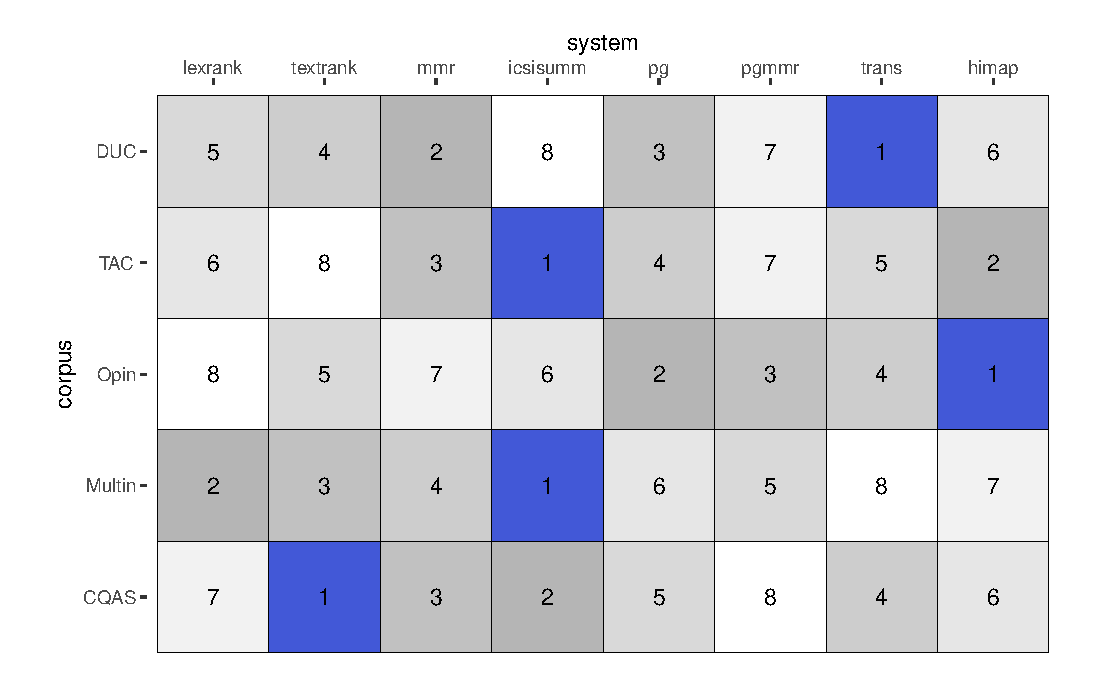
\includegraphics[width=\textwidth]{figures/results.eps}
    \caption{Overview based on the results from the initial paper, where for every MDS system performance over each dataset is ranked and the best performing system for every dataset is highlighted. Lower number means higher ROUGE-1 score.} \label{results}
\end{figure}


\end{document}